\documentclass[20pt]{article}
\usepackage[a4paper, top=3cm, left=3cm, right=2.5cm, bottom=2.5cm]{geometry}
\usepackage{lmodern}
\usepackage[T1]{fontenc}
\usepackage[portuguese]{babel}
\usepackage[utf8]{inputenc}
\usepackage{a4}
\usepackage[document]{ragged2e}
\usepackage{textgreek}
\usepackage{epstopdf}
\usepackage{graphicx}
\usepackage{fancyvrb}
\usepackage{amsmath}
\usepackage{float}
\usepackage{listings}
\usepackage{tabularx}


\begin{document}

\begin{titlepage}

\newcommand{\HRule}{\rule{\linewidth}{0.5mm}} % Defines a new command for the horizontal lines, change thickness here

\center % Center everything on the page

%----------------------------------------------------------------------------------------
%   HEADING SECTIONS
%----------------------------------------------------------------------------------------

\textsc{\LARGE Universidade do Minho}\\[1.5cm]
\HRule \\[0.4cm]

{ \huge \bfseries Programação em Lógica Estendida, Métodos de Resolução de Problemas e de Procura}\\[0.4cm]
\HRule \\[1.5cm]
\textsc{\Large Mestrado Integrado em Engenharia Informática}\\[0.5cm]
\textsc{\large Sistemas de Representação de Conhecimento e Raciocínio}\\[0.5cm]
\textsc{\large 2ºSemestre 2019/20}\\[0.5cm]


%----------------------------------------------------------------------------------------
%   AUTHOR SECTION
%----------------------------------------------------------------------------------------

\begin{minipage}{0.4\textwidth}
\begin{flushleft} \large
\emph{Author:}\\
Pedro Costa \\

\end{flushleft}
\end{minipage}
~
\begin{minipage}{0.4\textwidth}
\begin{flushright} \large
\emph{Docente:} \\
Paulo Novais\\
\end{flushright}
\end{minipage}\\[2cm]

%----------------------------------------------------------------------------------------
%   DATE SECTION
%----------------------------------------------------------------------------------------

{\large \today}\\[2cm]

%----------------------------------------------------------------------------------------
%   LOGO SECTION
%----------------------------------------------------------------------------------------

% \includegraphics[scale=0.3]{uminho}\\

%----------------------------------------------------------------------------------------

\vfill % Fill the rest of the page with whitespace

\end{titlepage}
\newpage
\tableofcontents
\newpage
\section{Introdução}

O relatório apresentado diz respeito ao trabalho proposto no âmbito da unidade curricular de Sistemas de Representação de Conhecimento e Raciocínio, utilizando uma linguagem de programação em lógica, PROLOG. 

Neste projeto, desenvolveu-se métodos de resolução de problemas e de procura aplicados a grafos. O objetivo foi, com base num dataset que contém informação sobre os autocarros de Oeiras, conseguir extrair informação relevante tal como caminhos mais curtos, escolher um mais pontos de intermédios para compor um caminho, entre vários outras opções.
\newpage

\section{Base de conhecimento}
Para representar a informação obtida nos datasets dados em forma de grafo, optei pela representação que me parecia mais simples. É obvio que se pode dividir um grafo em nodos e arestas, sendo exatamente isso que fiz. Assim, a minha base de conhecimento tem apenas dois axiomas, sendo estes:
\begin{itemize}
    \item \textbf{Stop}: Marca a existência de uma paragem com um conjunto de atributos, nomeadamente, id, latitude, longitude, estado de conservação, tipo de abrigo, se tem publicidade, operadora, lista de carreiras, código e nome de rua e freguesia onde se situa.
    \item \textbf{Connected}: Indica que existe uma conexão entre duas paragens, indicando ainda qual a carreira pelo qual esta conexão existe e ainda a distância entre as duas paragens.
\end{itemize}
Para obter a distância entre duas paragens utilizei o cálculo da distância euclidiana.

Para fazer o pré-processamento do dataset e transformá-lo nos axiomas descritos acima, elaborei um parser feito em Java que utiliza a biblioteca \textbf{ApachePOI} para fazer parse de excel. Percorri apenas os vários ficheiros, extraindo nodos dum e conexões do outro.

\textbf{Nota}: Considerei que qualquer conexão é bidirecional pois os autocarros conseguem fazer esse percurso em qualquer um dos sentidos.


\newpage
\section{Queries}
\subsection{Caminho entre dois nodos}
Para responder a esta query desenvolvi dois algoritmos diferentes de forma a poder comparar os resultados que obtia.

Um deles foi DFS (Depth-First Search) e o outro foi BFS (Breadth-First Search). 
Resultados obtidos para vários cenários:

\subsubsection{Trajeto entre 183 e 776}
Com BFS obtive a seguinte solução:

\vspace{1cm}
\begin{figure}[H]
    \centering
    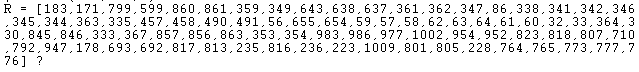
\includegraphics[scale=0.8]{images/bfs_183_776.png}
    \caption{Trajeto obtido com BFS entre 183 e 776}
\end{figure}

Com DFS não foi possível obter uma solução em tempo decente. Isto acontece em vários cenários pois recursividade num grande conjunto de dados com algoritmos não otimizados torna extremamente difícil de obter soluções ocasionalmente.

\subsubsection{Trajeto entre 183 e 79}
Com BFS obtive a seguinte solução:

\vspace{1cm}
\begin{figure}[H]
    \centering
    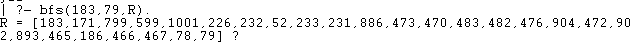
\includegraphics[scale=0.8]{images/bfs_183_79.png}
    \caption{Trajeto obtido com BFS entre 183 e 79}
\end{figure}

Com DFS obteve-se um caminho mais longo mas que acontece ao longo duma carreira diretamente:

\vspace{1cm}
\begin{figure}[H]
    \centering
    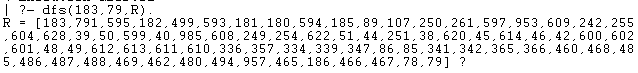
\includegraphics[scale=0.8]{images/dfs_183_79.png}
    \caption{Trajeto obtido com DFS entre 183 e 79}
\end{figure}

\newpage
\subsection{Caminho entre dois nodos com apenas certas operadoras}
\begin{verbatim}
pathOps(Origin,Destiny,Ops,Path) :- pathOpsAux(Origin,[Destiny],Ops,Path).
pathOpsAux(Origin,[Origin|P1],_,[Origin|P1]).
pathOpsAux(Origin,[Y|P1],Ops,Path) :-   connectedBiDir(X,Y,C,_),
                                stop(X,_,_,_,_,_,Operator,_,_,_,_),
                                stop(Y,_,_,_,_,_,OperatorY,_,_,_,_),
                                member(Operator,Ops),
                                member(OperatorY,Ops),
                                \+ memberchk(X,[Y|P1]), 
                                pathOpsAux(Origin,[X,(Y,OperatorY,C)|P1],Ops,Path). 
\end{verbatim}

Trajeto entre 745 e 107 com as operadoras Vimeca e SCoTTURB:
\vspace{1cm}
\begin{figure}[H]
    \centering
    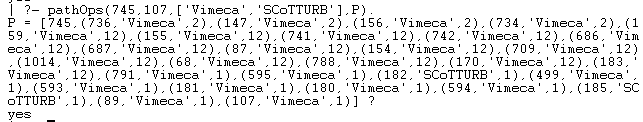
\includegraphics[scale=0.8]{images/trajeto_vim_scot_745_107.png}
    \caption{Trajeto obtido com DFS entre 745 e 107 apenas usando as operadoras vimeca e scotturb}
\end{figure}

\newpage
\subsection{Caminho entre dois nodos excluindo certas operadoras}
\begin{verbatim}
pathWithoutOperators(Origin,Destiny, Operators, Path) :-
    pathWithoutOperatorsAux(Origin,[Destiny],Operators,Path).
pathWithoutOperatorsAux(Origin,[Origin|P1],_,[Origin|P1]).
pathWithoutOperatorsAux(Origin,[Y|P1],Operators,Path) :- connectedBiDir(X,Y,C,_),
                                                        stop(X,_,_,_,_,_,Operator,_,_,_,_),
                                                        \+ member(Operator,Operators),
                                                        \+ memberchk(X,[Y|P1]), 
                                                        pathWithoutOperatorsAux(Origin,[X,Y,(Operator,C)|P1],Operators,Path).       
\end{verbatim}

Trajeto entre 954 e 58 excluindo a operadora Vimeca.
\vspace{1cm}
\begin{figure}[H]
    \centering
    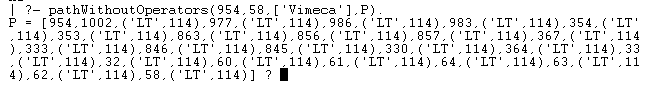
\includegraphics[scale=0.8]{images/no_ops_954_58.png}
    \caption{Trajeto obtido com DFS entre 954 e 58 sem usar a operadora Vimeca}
\end{figure}

\newpage
\subsection{Paragens com maior número de carreiras num determinado percurso }
Para responder a esta query percorro o percurso que me é dado e agrupo cada id da lista com o número de paragens correspondentes. De seguida, utilizo uma função auxiliar que mantém apenas os maiores segundos valores duma lista de pares.

\begin{verbatim}
most_tracks(Path, NTracks) :- 
    most_tracks_aux(Path, [], AccNTracks), 
    biggest_pairs(AccNTracks, NTracks).
most_tracks_aux([],[P|T1],[P|T1]).
most_tracks_aux([P|T1], Acc, NTracks) :- stop(P,_,_,_,_,_,_,Tracks,_,_,_),
                                         length(Tracks, L),                                
                                         most_tracks_aux(T1,[(P,L)|Acc],NTracks).                    

biggest_pairs(L,R) :- maxList(L,K,R).

maxList([],(_,0),L).
maxList([(P1,P2)|Tail],(M1,M2),[(M1,M2)]) :- 
    maxList(Tail,(TM1,TM2),_), 
    P2 > TM2, 
    M1 is P1, 
    M2 is P2.
maxList([(P1,P2)|Tail],(M1,M2),L) :- 
    maxList(Tail,(TM1,TM2),L), 
    P2 < TM2, 
    M1 is TM1, 
    M2 is TM2.
maxList([(P1,P2)|Tail],(M1,M2),[H,(P1,P2)|L]) :- 
    maxList(Tail,(TM1,TM2),[H|L]), 
    P2 == TM2, 
    M1 is TM1, 
    M2 is TM2.
\end{verbatim}

Paragens com maior número de carreiras num percurso entre 183 e 250:
\vspace{1cm}
\begin{figure}[H]
    \centering
    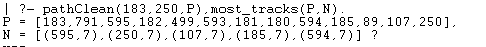
\includegraphics[scale=0.8]{images/most_tracks_183_250.png}
    \caption{Trajeto obtido com DFS entre 183 e 250 e paragens com maior número de carreiras}
\end{figure}

\newpage
\subsection{Percurso com menor número de paragens}
Para responder a esta query apenas percorro todos os trajetos obtidos com DFS/BFS e escolho o que têm menos paragens.

\begin{verbatim}
shortest_in_stops(Origin,Destiny,Path) :- 
    bfs(Origin, Destiny, Path),
    \+ (bfs(Origin, Destiny, Path2),
    length(Path, L1),
    length(Path2, L2),
    Path2 \= Path,
    L2 =< L1).    
\end{verbatim}

Menor número de paragens obtido entre 499 e 78:
 \vspace{1cm}
\begin{figure}[h]
    \centering
    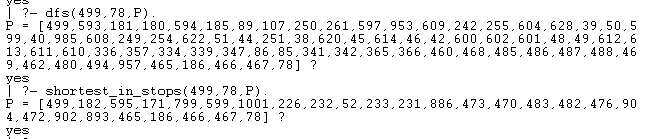
\includegraphics[scale=0.8]{images/less_stops_499_78.png}
    \caption{Trajetos obtidos entre 499 e 78 (DFS versus Algoritmo de cima)}
\end{figure}

\newpage
\subsection{Percurso com menor distância}
Para responder a esta query apenas percorro todos os trajetos obtidos com DFS/BFS e escolho o que têm a menor distância total.

\begin{verbatim}
fastest(Origin,Destiny,MinDist,Path) :- 
    pathWithDistance(Origin, Destiny, MinDist, Path),
    \+ (pathWithDistance(Origin, Destiny, LowerDist, Path2),
    Path2 \= Path,
    LowerDist =< MinDist). 
\end{verbatim} 

\newpage
\subsection{Percurso que passe apenas por paragens com publicidade}
Este exercício foi resolvido com uma implementação adaptada dum algoritmo do estilo de DFS.

\begin{verbatim}
withAdvertisingOnlyPath(Origin,Destiny, Path) :-    
    withAdvertisingOnlyPathAux(Origin,[Destiny],Path).
withAdvertisingOnlyPathAux(Origin,[Origin|P1],[Origin|P1]).
withAdvertisingOnlyPathAux(Origin,[Y|P1],Path) :-   
    connectedBiDir(X,Y,C,_),
    stop(X,_,_,_,_,true,Operator,_,_,_,_),
    \+ memberchk(X,[Y|P1]), 
    withAdvertisingOnlyPathAux(Origin,[X,Y,(Operator,C)|P1],Path).      
\end{verbatim}

Abaixo pode-se ver que entre 174 e 274 não existe um caminho que passe apenas por paragens com publicidade. Pode-se ainda ver que entre existe um caminho que passa apenas por paragens com publicidade entre 268 e 378.

 \vspace{1cm}
\begin{figure}[h]
    \centering
    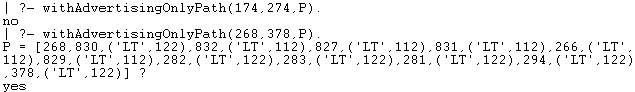
\includegraphics[scale=0.8]{images/advertising.png}
\end{figure}

\newpage
\subsection{Percurso que passe apenas por paragens abrigadas}
Esta query tem exatamente o mesmo estilo que a anterior apenas mudando a condição imposta.
\begin{verbatim}
shelteredPath(Origin,Destiny, Path) :-  
    shelteredPathAux(Origin,[Destiny],Path).
shelteredPathAux(Origin,[Origin|P1],[Origin|P1]).
shelteredPathAux(Origin,[Y|P1],Path) :-
    connectedBiDir(X,Y,C,_),
    stop(X,_,_,_,'Fechado dos Lados',_,Operator,_,_,_,_),
    \+ memberchk(X,[Y|P1]), 
    shelteredPathAux(Origin,[X,Y,(Operator,C)|P1],Path).    
\end{verbatim}

Trajeto com paragens abrigadas entre 323 e 491:
 \vspace{1cm}
\begin{figure}[h]
    \centering
    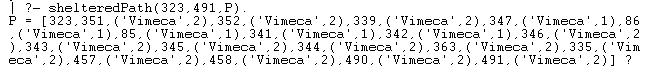
\includegraphics[scale=0.8]{images/sheltered_path.png}
    \caption{Trajeto com paragens abrigadas entre 323 e 491}
\end{figure}

\newpage
\subsection{Percurso que passa por um ou mais pontos intermédios}
Nesta query tirei partido duma função que remove um ponto intermédio da lista que queremos satisfazer e procuro um trajeto até essa lista terminar e se chegar ao nodo de destino.

\begin{verbatim}
withIntermediate(Origin,Destiny, Intermediate, Path) :-
withIntermediateAux(Origin,[Destiny],Intermediate,Path).
withIntermediateAux(Origin,[Origin|P1],[],[Origin|P1]).
withIntermediateAux(Origin,[Y|P1],Intermediate,Path) :- 
    connectedBiDir(X,Y,C,_),
    stop(X,_,_,_,_,_,Operator,_,_,_,_),
    member(X,Intermediate),
    delete_1(X,Intermediate, New),
    \+ memberchk(X,[Y|P1]), 
withIntermediateAux(Origin,[X,Y,(Operator,C)|P1],New,Path).     
withIntermediateAux(Origin,[Y|P1],Intermediate,Path) :- 
    connectedBiDir(X,Y,C,_),
    stop(X,_,_,_,_,_,Operator,_,_,_,_),
    \+member(X,Intermediate),
    \+ memberchk(X,[Y|P1]), 
    withIntermediateAux(Origin,[X,Y,(Operator,C)|P1],Intermediate,Path).    
\end{verbatim}

\newpage
\section{Pesquisa informada}
\subsection{Variação do algoritmo guloso para obter o caminho mais longo}
Para obter este algoritmo tirei partimo da seguinte função heuristica que é capaz de determinar entre dois nodos o que encontra mais perto do destino final:
\begin{verbatim}
estima(Nodo,Destino,Dist) :- 
    stop(Nodo,LatX,LonX,_,_,_,_,_,_,_,_),
    stop(Destino,LatY,LonY,_,_,_,_,_,_,_,_),
    Lat is (LatX - LatY) * (LatX - LatY), 
    Lon is (LonX - LonY) * (LonX - LonY), 
    Dist is sqrt(Lat+Lon).
\end{verbatim}

Assim, torna-se possível escolher a melhor solução dentro do conjunto de nodos ligados ao nodo que estamos a explorar em cada iteração. Tiro partido duma lista com prioridade para ordenar os nodos por interesse, garantindo assim que escolho sempre o caminho mais distante.

No final, removemos os nodos repetidos da lista dos obtidos (devido à existência do mesmo nodo em carreiras diferentes acabamos por ter muitos repetidos a ser tidos em conta desnecessariamente) e invertemos a lista para ficar num sentido de início para fim.

Uma aplicação deste algoritmo podia ser, por exemplo, desenvolver um passeio turístico por Oeiras.

Comparação entre um percurso de 183 a 766 obtido com BFS e por o algoritmo descrito acima:
 \vspace{1cm}
\begin{figure}[h]
    \centering
    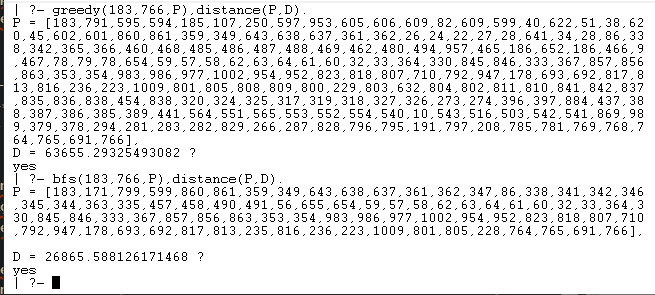
\includegraphics[scale=0.8]{images/greedy_183_766.png}
\end{figure}

Como se pode ver, o percurso obtido pelo greedy é extremamente mais longo que o obtido pelo BFS.

\newpage
\section{Conclusão}
Concluindo, foi interessante realizar este trabalho pois permitiu explorar um estilo de programação diferente do que estou habituado. 

No entanto, não faço um balanço positivo da exeperiência. Isto deve-se, muito provavelmente, à minha inexperiência com programação em lógica. Digo que faço um balanço negativo uma vez que grande parte dos algoritmos desenvolvidos são incapazes de descobrir uma solução para paragens que não tenham sido escolhidas pre-meditamente.

Acredito, definitivamente, que se tivessem sido desenvolvidos algoritmos mais eficientes o problema acima não se verificaria. 
